\begin{figure}[ht!]
    \centering
    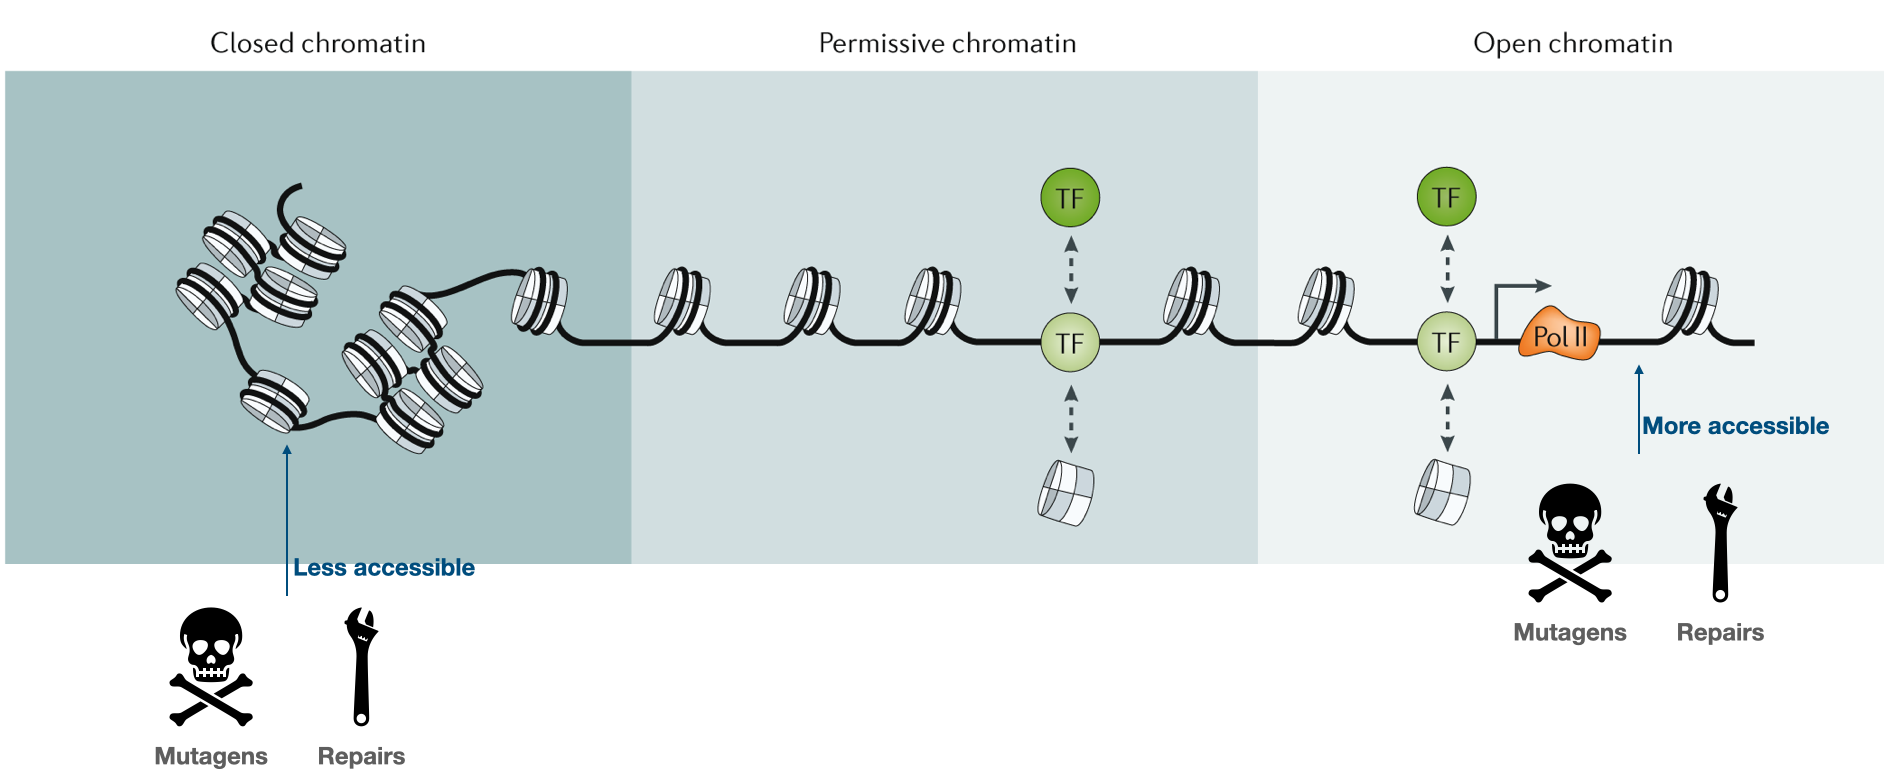
\includegraphics[scale=0.24]{graphics/chromatin_demo.png}
\caption{}
    % \caption{\textbf{The distribution of mutations across the genome is hypothesised to be influenced by cell chromatin structure.} DNA in closed chromatin regions is less accessible to mutagens and DNA repair, and is more prone to mutations. Different cell types have different chromatin structures as well as different repair systems, making the genomic location of mutations a potential source for distinguishing cancers.  TF means transcription factor, Pol II means polymerase II. Figure modified from \citet{Klemm2019ChromatinEpigenome}.}
    \label{fig:chromatin_demo}
\end{figure}
